\documentclass{beamer}
\usepackage{graphicx}
\usepackage{amsmath}

\title{Monetary and Fiscal Policy Analysis --- December 16, 2008}
\author{Anuj Patel, Charles Ancel, and Henry Szklanny (Team Two)}
\date{August 2nd, 2024}

\begin{document}

\frame{\titlepage}

\section{Introduction}
\begin{frame}
    \frametitle{Identity Verification}
    My name is Charles Ancel, my UIN is 654604114, and this is my ID\@. I'm currently enrolled in ECON 425 during the Summer Session. This assignment is part of the requirement from the University regarding the College of LAS's identity verification policy for LAS Online-certified classes. For the answers in this assignment, I did not use any form of Artificial Intelligence (AI) help, such as Chat-GPT or similar, and thus my answers will accurately and fairly reflect my own learning from this course.
\end{frame}
\begin{frame}
    \frametitle{Introduction}
    Good evening, everyone. My name is Charles Ancel, and today I will be presenting an analysis of the monetary and fiscal policy decisions around December 16, 2008. I am presenting on behalf of Team Two, which includes Anuj Patel, Charles Ancel, and Henry Szklanny. This presentation is part of ECON 425, a course on Macroeconomic Policy at the University of Illinois. Let's dive in.
\end{frame}



\section{Contextual Information}
\begin{frame}
    \frametitle{Contextual Information}
    To set the stage, the Federal Open Market Committee (FOMC) had recently lowered the federal funds rate by 50 basis points to 1\% in response to slowing economic activity. On December 1st, the National Bureau of Economic Research officially declared that the US had entered a recession.
    \newline
    
    Key indicators showed significant declines in retail sales, manufacturing, real estate purchases, and business and consumer lending. Labor markets were weakening, price pressures were decreasing, and financial markets were experiencing further declines as pessimism grew. The economy was projected to see a 5\% fall in GDP over the next two quarters, with unemployment rising to about 8\% in 2010 and PCE inflation remaining around 1\% for 2009 and 2010.
\end{frame}

\section{Contextual Data}
\begin{frame}
    \frametitle{Contextual Data --- GDP}
    Let's take a closer look at the GDP data from Q4 2003 to Q4 2013. During this period, the US economy was in a recession. By the end of Q4 2008, GDP was approximately 14,608.209 billion USD\@.
\end{frame}

\begin{frame}
    \frametitle{Graph --- GDP}
    \begin{figure}[h!]
        \centering
        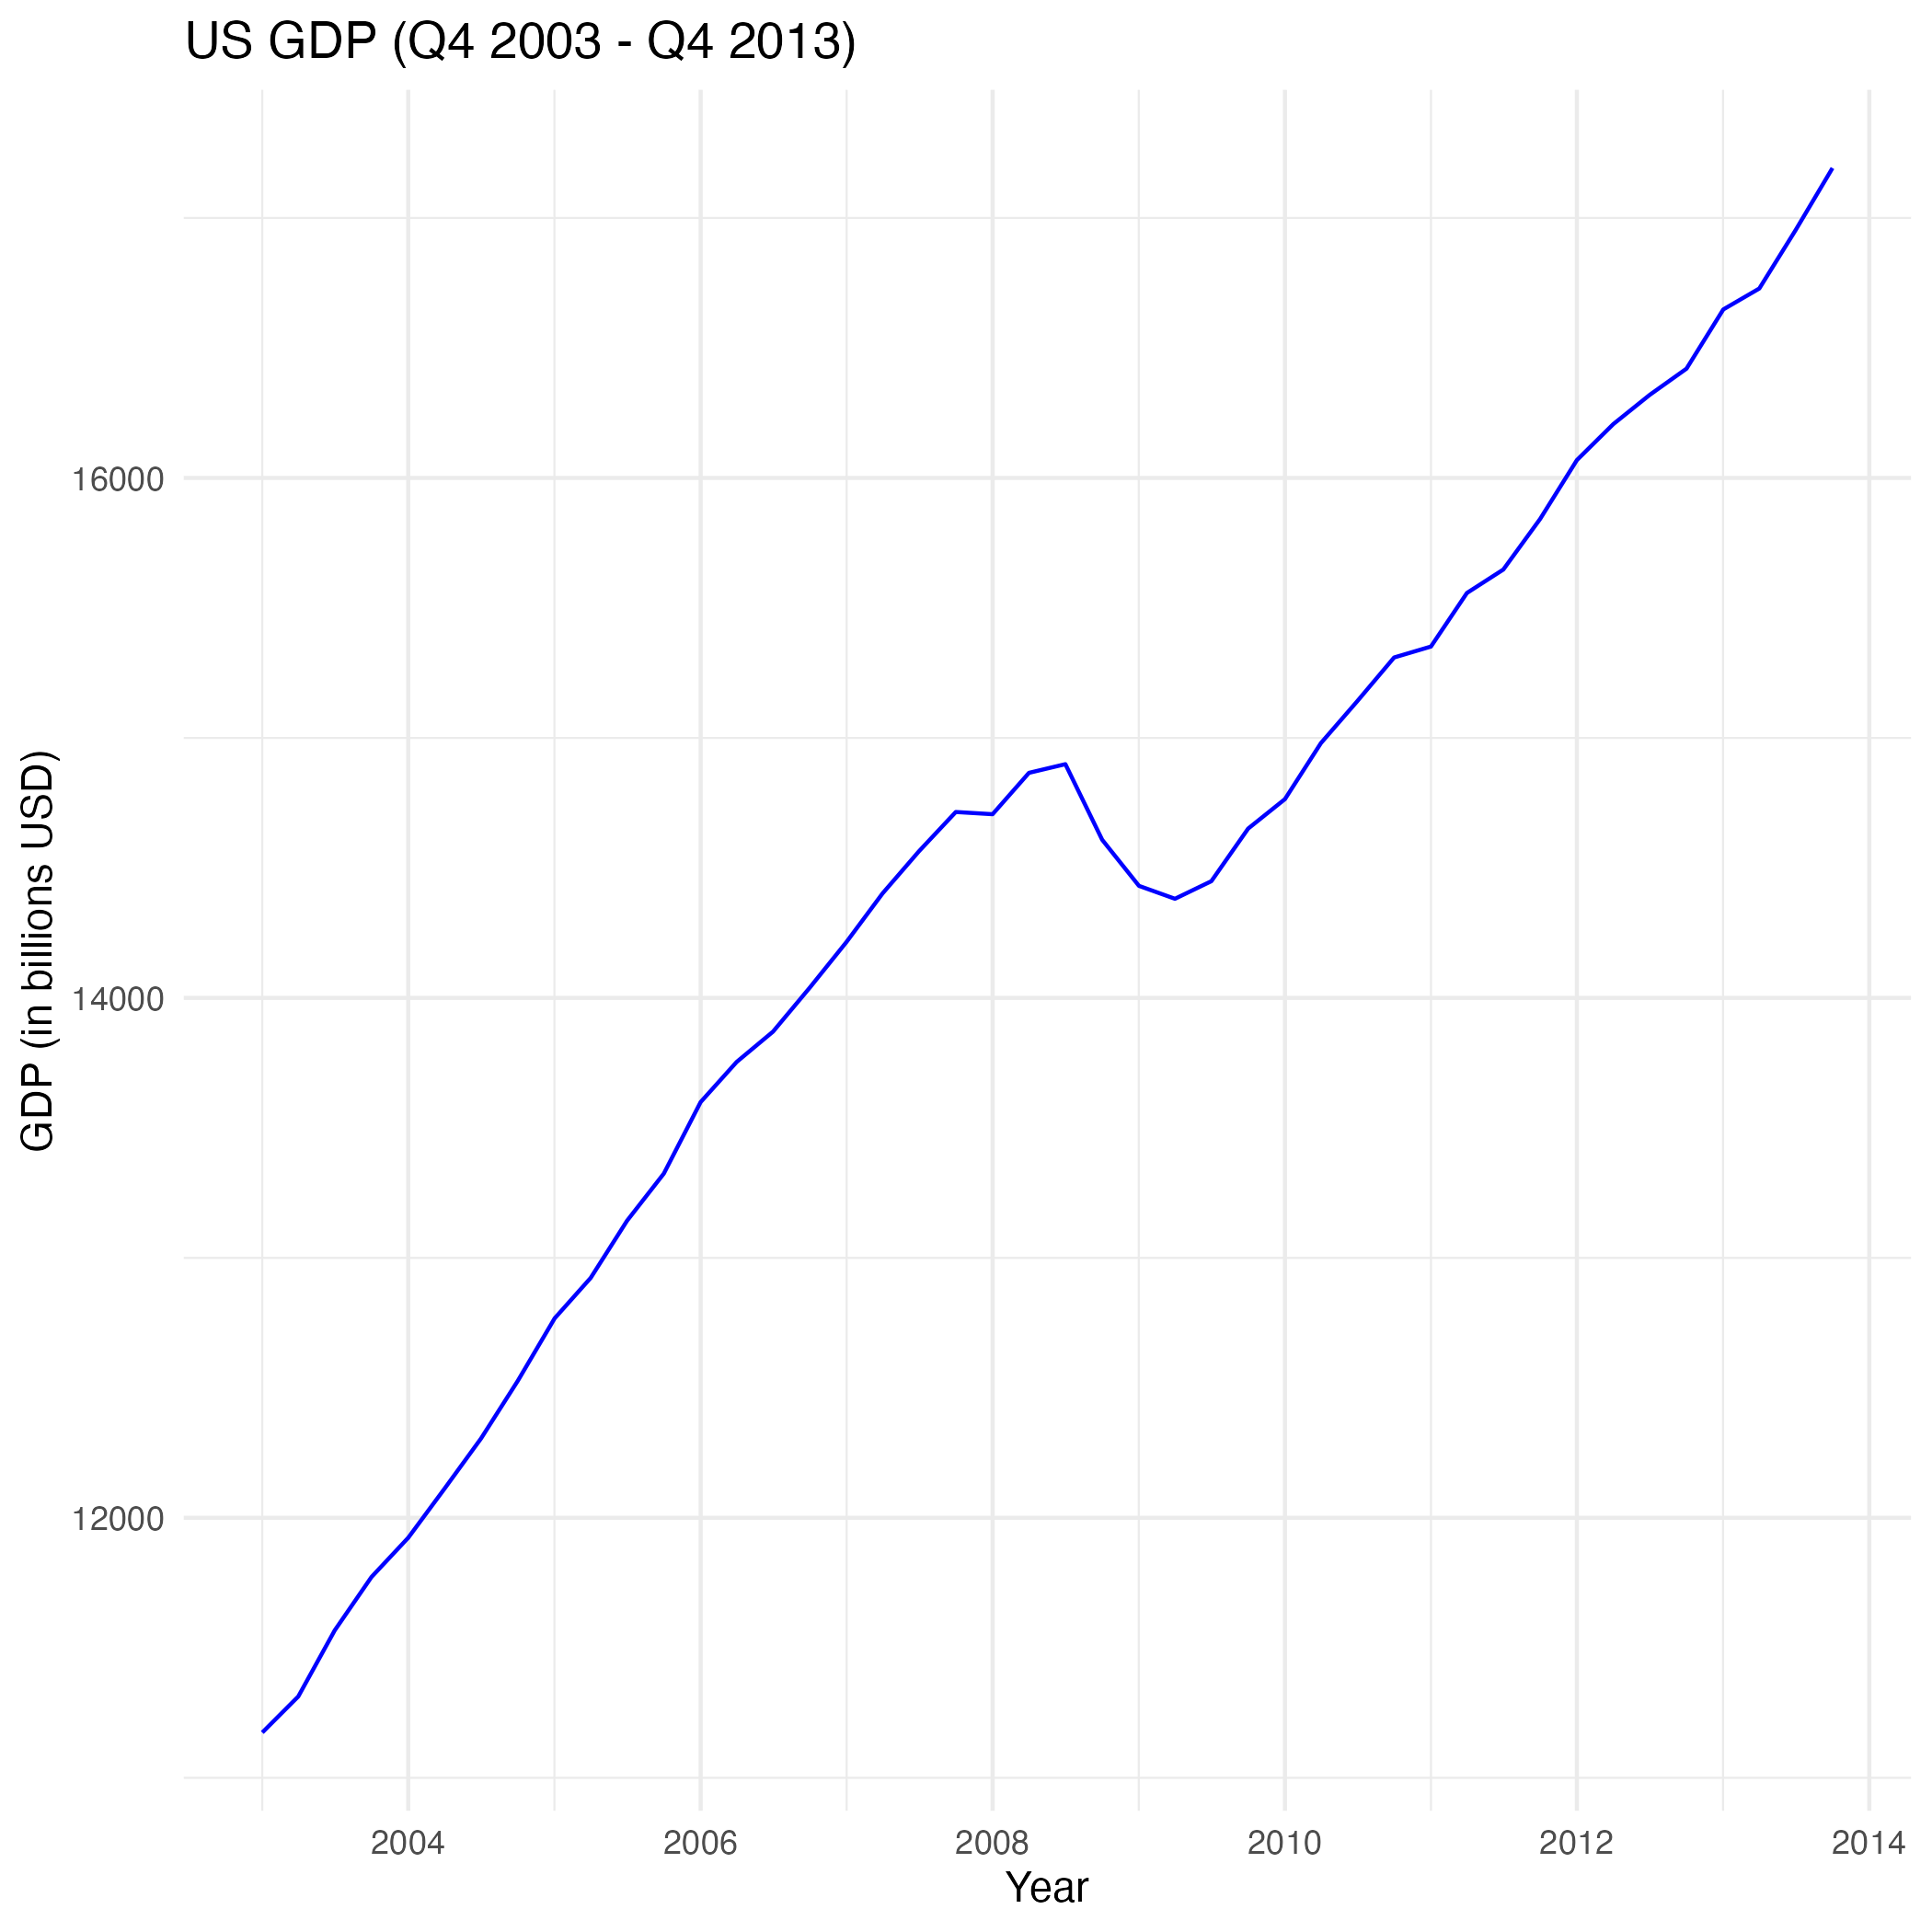
\includegraphics[width=0.8\textwidth]{/Users/cancel/Personal/Coursework/Econ425/FinalWork/R/gdp_graph.png}
    \end{figure}
\end{frame}

\begin{frame}
    \frametitle{Explanation --- GDP}
    As you can see from the graph, the recession's impact on GDP is quite evident. There was a significant decline during the period of interest. This decline highlights the severity of the economic downturn and underscores the importance of implementing monetary policies aimed at stabilizing the economy and promoting recovery.
\end{frame}

\begin{frame}
    \frametitle{Contextual Data --- Inflation}
    Next, we examine inflation as measured by the Consumer Price Index (CPI). This metric reflects the annual percentage change in the cost of a basket of goods and services. During this period, inflation dropped dramatically, even becoming negative at some point in 2009.
\end{frame}

\begin{frame}
    \frametitle{Graph --- Inflation}
    \begin{figure}[h!]
        \centering
        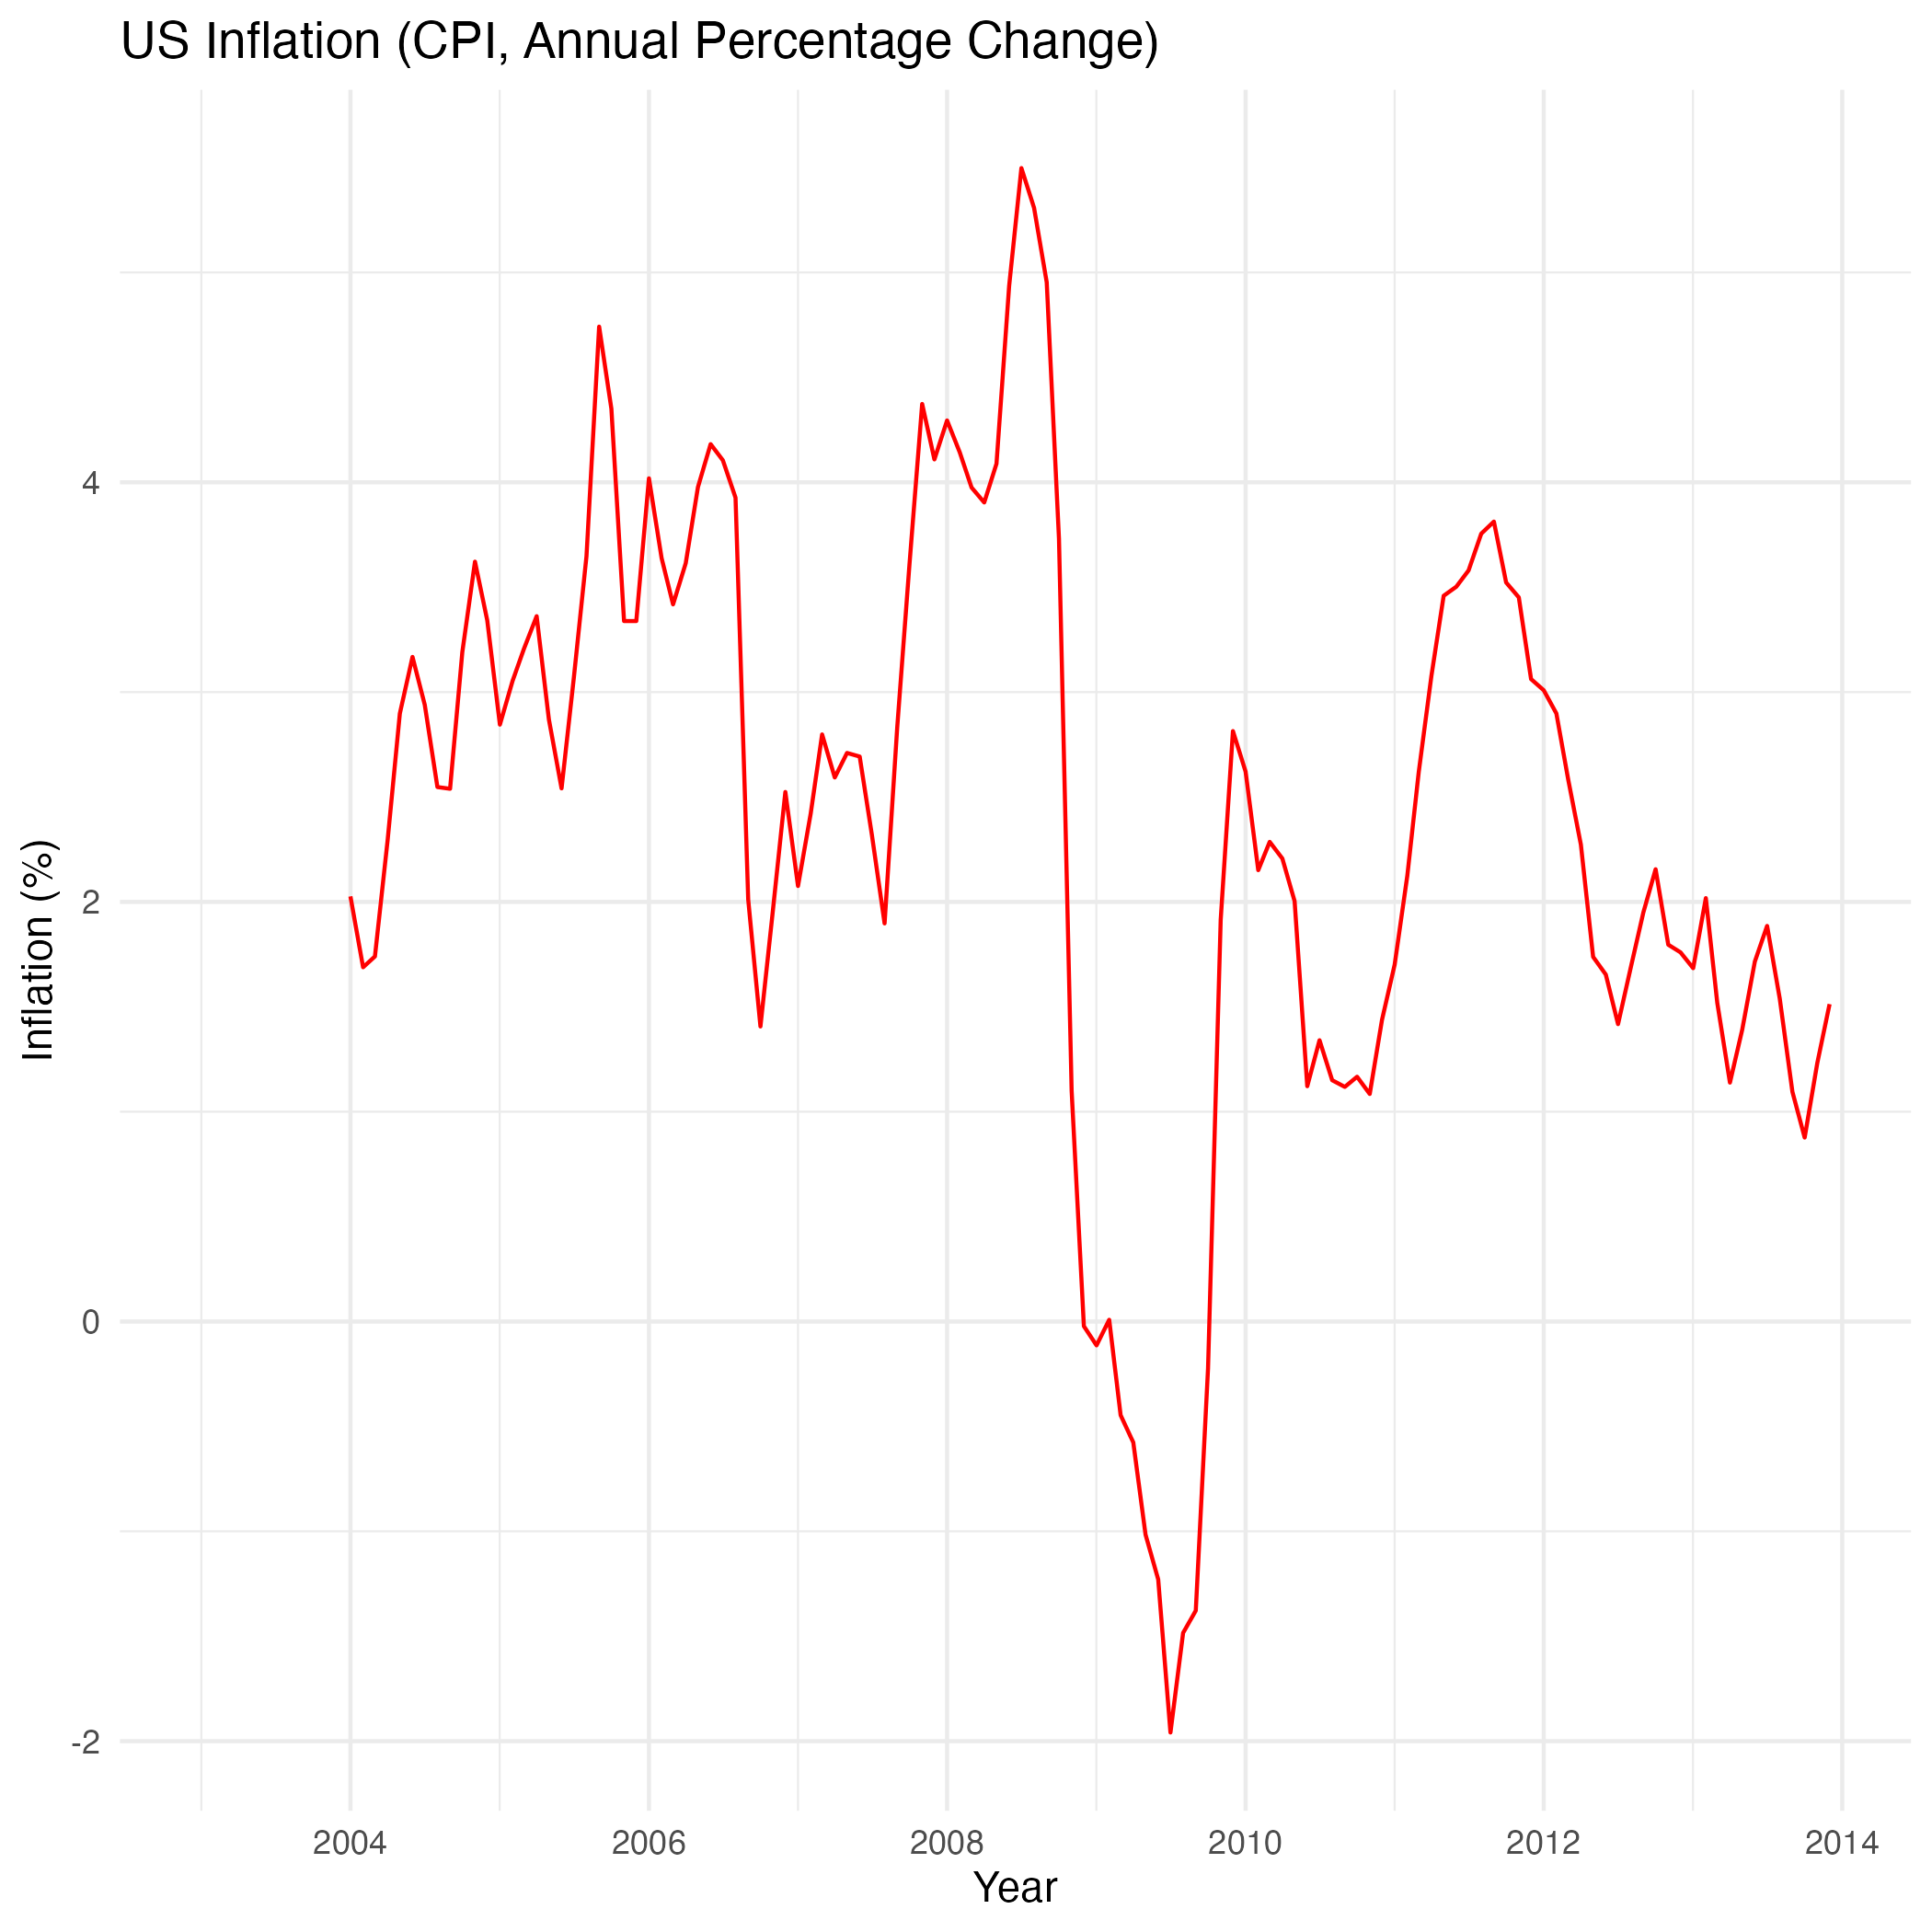
\includegraphics[width=0.8\textwidth]{/Users/cancel/Personal/Coursework/Econ425/FinalWork/R/inflation_graph.png}
    \end{figure}
\end{frame}

\begin{frame}
    \frametitle{Explanation --- Inflation}
    This graph shows the sharp decline in inflation, highlighting the deflationary pressures faced by the economy during the recession. Negative inflation, or deflation, can lead to reduced consumer spending as people delay purchases in anticipation of lower prices, further exacerbating economic downturns.
\end{frame}

\begin{frame}
    \frametitle{Contextual Data --- Interest Rates}
    Now, let's look at the federal funds effective rate from 2003 to 2013. There were significant rate cuts during this period, resulting in extended near-zero rates. This strategy aimed to stimulate the economy by making borrowing cheaper and encouraging spending and investment.
\end{frame}

\begin{frame}
    \frametitle{Graph --- Interest Rates}
    \begin{figure}[h!]
        \centering
        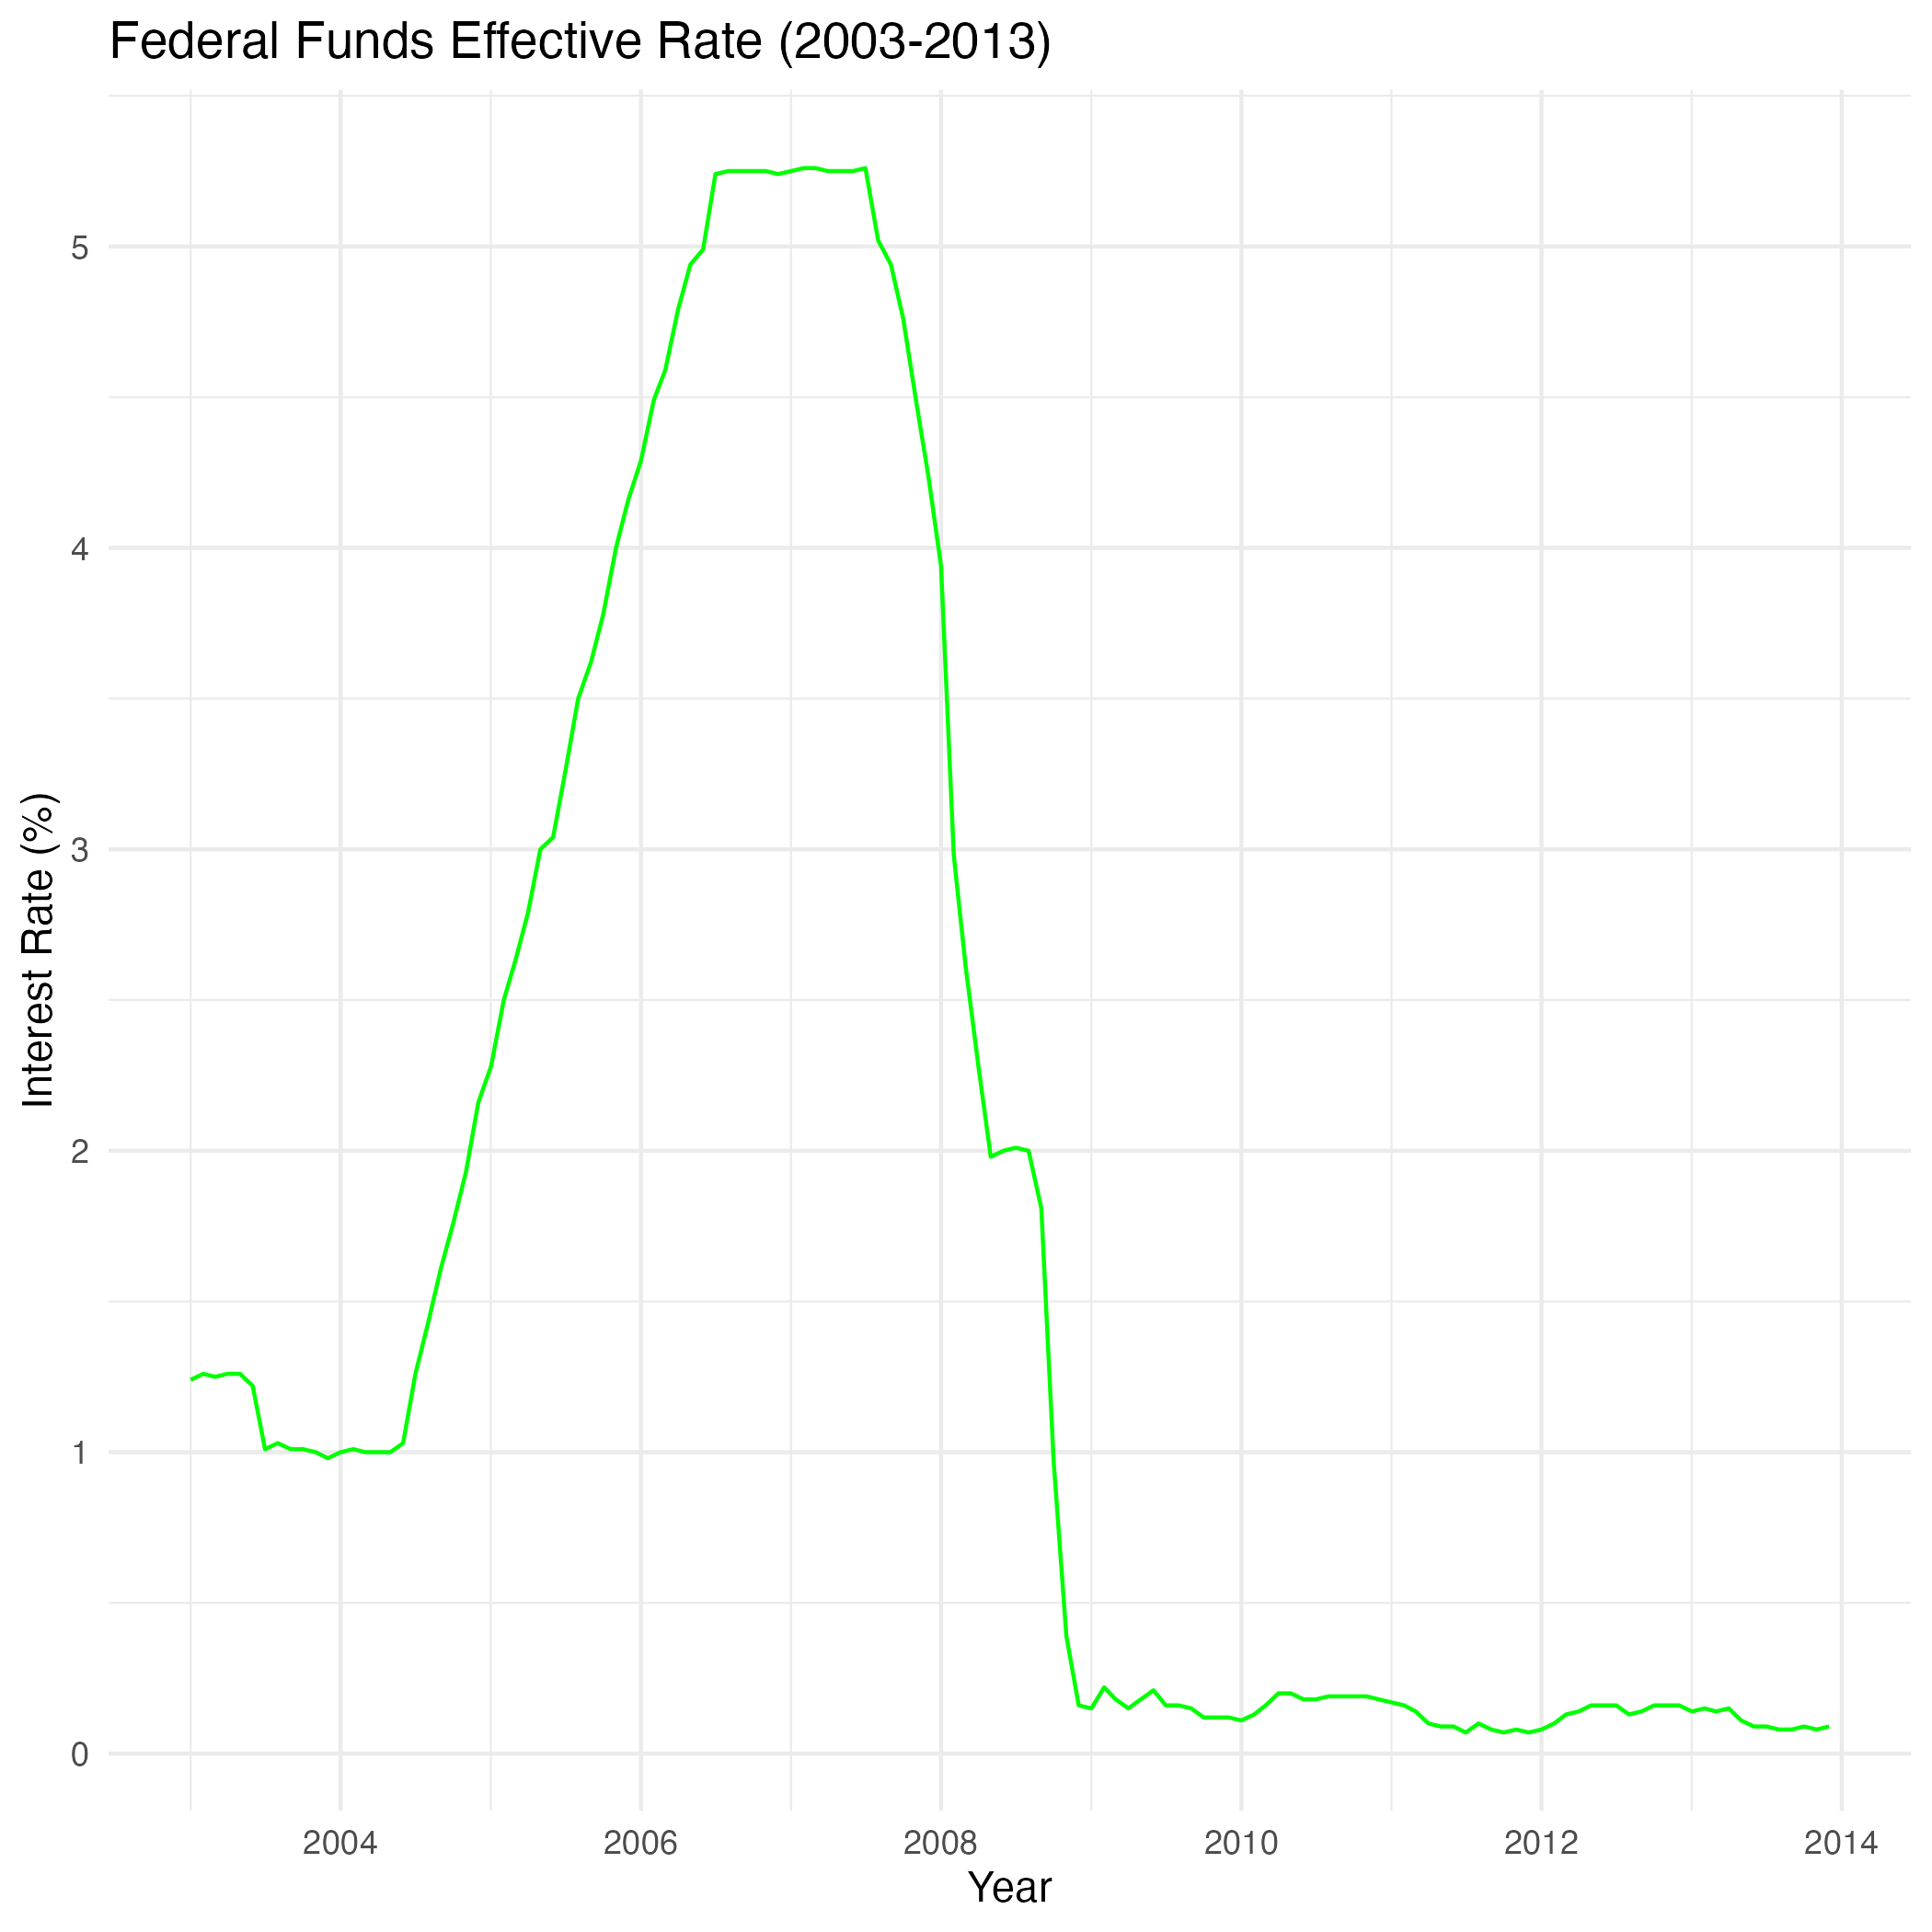
\includegraphics[width=0.8\textwidth]{/Users/cancel/Personal/Coursework/Econ425/FinalWork/R/interest_rate_graph.png}
    \end{figure}
\end{frame}

\begin{frame}
    \frametitle{Explanation --- Interest Rates}
    Here, we can see the drastic reduction in interest rates, which remained near zero for an extended period. Such low interest rates were intended to boost economic activity by lowering the cost of borrowing, thereby encouraging both consumer spending and business investments.
\end{frame}

\begin{frame}
    \frametitle{Contextual Data --- Unemployment Rate}
    Lastly, we examine the unemployment rate from 2003 to 2013. Before the recession, the unemployment rate was steady around 5\%. However, it peaked at 10\% in October 2009, indicating the severe impact of the recession on the labor market.
\end{frame}

\begin{frame}
    \frametitle{Graph --- Unemployment Rate}
    \begin{figure}[h!]
        \centering
        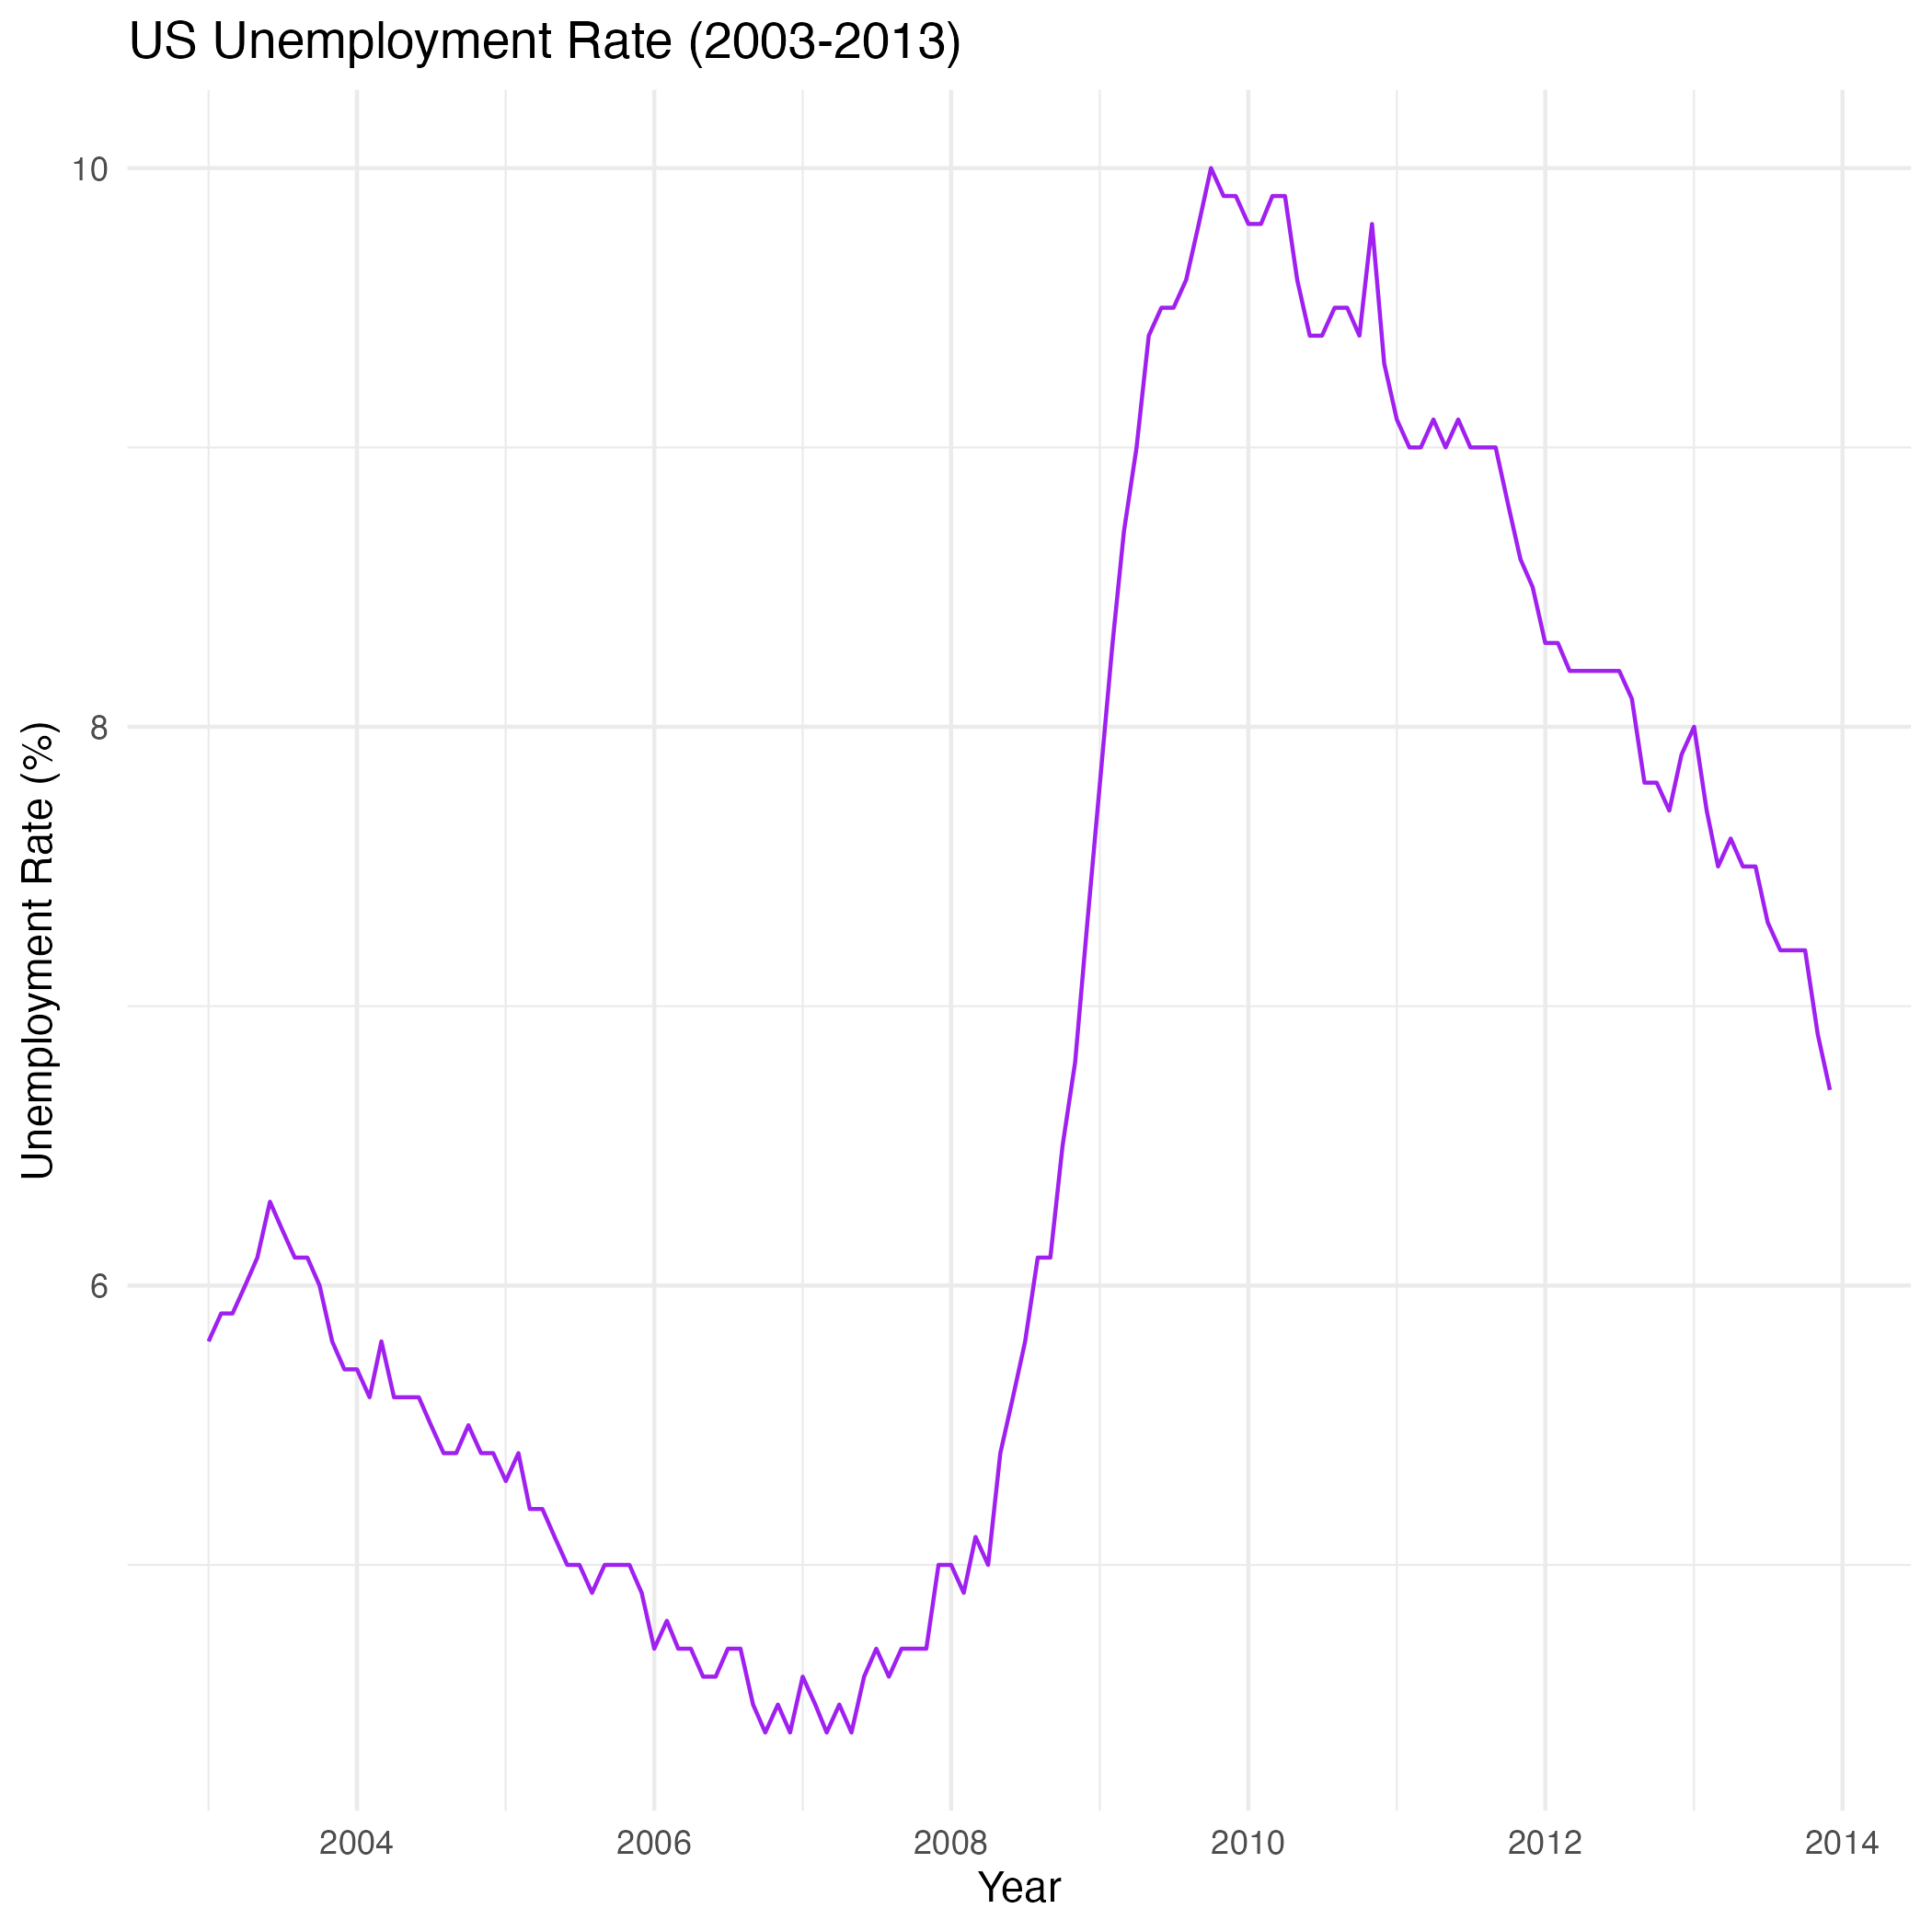
\includegraphics[width=0.8\textwidth]{/Users/cancel/Personal/Coursework/Econ425/FinalWork/R/unemployment_rate_graph.png}
    \end{figure}
\end{frame}

\begin{frame}
    \frametitle{Explanation --- Unemployment Rate}
    The graph clearly illustrates the significant rise in unemployment during the recession, peaking in late 2009. This increase in unemployment reflects the widespread job losses and economic hardships faced by many individuals, underscoring the need for effective monetary and fiscal policies to support recovery.
\end{frame}

\section{Theory and Decision}
\begin{frame}
    \frametitle{Theory and Decision}
    In the middle of the housing market crisis of 2008 and 2009, we recommended lowering the federal funds rate to around 0.5\% ± 0.25\%. The rationale behind this decision was to stimulate consumer spending and investment by making borrowing cheaper, counteracting deflationary pressures, and supporting economic recovery.
    \newline
    
    We also considered implementing a zero interest rate policy and providing effective forward guidance to ensure transparency and manage market expectations.
\end{frame}

\section{Statement}
\begin{frame}
    \frametitle{Statement}
    The Federal Open Market Committee decided today to lower its target for the federal funds rate by 50 basis points to 0.5 percent. Contributing to this decision has been the continued decline of many economic indicators. In particular, a marked deterioration of labor markets and industrial production have led to a bleak outlook. At the same time, prices have continued to decline, and we now project inflation to be at 1 percent for the next couple of years. In spite of this, the Committee believes that the economy will stabilize in the coming year with the implementation of a new stimulus package. The Fed will continue to closely monitor the economy and reaffirms its promise to ensure economic growth and price stability. If necessary, the Fed is willing to further lower the federal funds rate and maintain a lower interest rate for an extended period to reach this goal.
\end{frame}

\section{Comparison with Fed's Decision}
\begin{frame}
    \frametitle{Comparison with Fed's Decision}
    Comparing our decision with the Fed's actual decision, the Fed set a target range of 0--0.25\%, which was more aggressive than our recommended target of 0.5\%. The Fed's decision was likely influenced by the need to provide a stronger immediate boost to the economy during such a critical period.
    \newline
    
    Additionally, the Fed implemented extra policies to support mortgage and housing markets and facilitate credit extension to households and small businesses. Given the worsening economic indicators, the Fed's more impactful decision was likely more effective.
\end{frame}

\section{Conclusions}
\begin{frame}
    \frametitle{Conclusions}
    In conclusion, the analysis of the economic conditions in December 2008 highlighted the severity of the recession, with significant declines in GDP and increases in unemployment. Our recommended monetary policy aimed to stimulate economic activity by lowering interest rates and providing forward guidance. However, the Fed's more aggressive approach was likely more effective in providing the necessary economic boost.
    \newline
    
    This exercise underscores the importance of flexibility and responsiveness in monetary policy, particularly during times of economic crisis. Future policymakers should consider the potential benefits of more aggressive measures when faced with similar challenges.
\end{frame}

\section{Q\&A}
\begin{frame}
    \frametitle{Q\&A}
    Thank you for your attention. This concludes my presentation on the monetary and fiscal policy decisions of December 2008. I hope this has provided a clear understanding of the economic context and the rationale behind policy decisions. If you have any questions, please feel free to ask.
\end{frame}

\end{document}
